\chapter{Moteur de combats}



% Tout d'abord pour comprendre comment la génération de vaisseaux fonctionne, il faut comprendre comment un vaisseau est représenté. 
% Ensuite, pour déterminer le meilleur vaisseau, nous avons appliqué plusieurs méthodes connues d'optimisation que nous allons expliquer. 


	\section{Représentation des vaisseaux}
	
	On peut distinguer deux types de représentations qui sont complémentaires. En premier lieu il y a la représentation des vaisseaux de base, ensuite il y a la représentation des vaisseaux personnalisés, c'est-à-dire les vaisseaux auxquels on a ajouté ou enlevé des armes, améliorations, etc. \\
	
	Dans la représentation de base on stocke différentes données :
	\begin{itemize}
		\item les systèmes présents et leurs niveaux de base (c'est-à-dire le nombre maximal d'énergie que l'on peut mettre dedans) ;
		\item les armes, les drones et les améliorations ;
		\item les salles avec : leurs coordonnées, le système qui est dedans ou celui qui peut être dedans, les portes, les membres d'équipage.
	\end{itemize}
	\ 
	
	Ensuite, dans la représentation des vaisseaux personnalisés, on stocke les ajouts et suppressions d'équipement. Ces ajouts et suppressions correspondent aux interactions possibles que l'on peut avoir dans les magasins dans le jeu original.

	\section{Le déroulement d'un combat}

	Nous avons décidé de gérer un combat avec un fonctionnement au tour par tour tout en gardant un faible temps entre chaque tour. 
	Cela nous permet de gérer les phases d'attaques et de cooldowns indépendamment, tout en restant proche du jeu original qui se déroule en temps réel.

	Le vaisseau gagnant est celui qui n'est pas mort ou celui qui a le plus de vie au bout de 5 secondes. Si les deux vaisseaux ont le même nombre de points de vie, c'est le vaisseau numéro 1 qui est désigné gagnant. Un combat dure en moyenne haute 2 secondes, 5 secondes permettent donc des combats plus longs entre des vaisseaux bien équipés.

		
		\subsection{Le déroulement d'une attaque}

			\paragraph{L'utilisation d'une arme} 

			Pour chaque arme, la même procédure va être appliquée. Celle-ci est gérée par le système des armes.
			\begin{figure}[H]
				\caption{Début de l'utilisation d'une arme}
				\label{fig:startAttackWeapon}
				\centering
				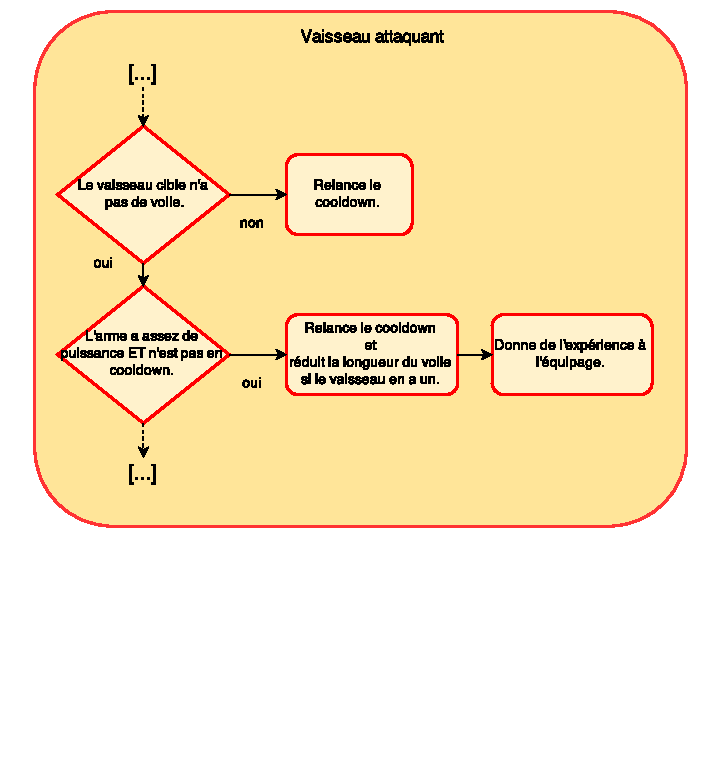
\includegraphics[width=0.85\linewidth]{attackSequenceStart.pdf}
			\end{figure}
			Comme décrit sur la figure~\ref{fig:startAttackWeapon}, le système fait d'abord tous les préparatifs avant d'être sûr qu'il a le droit d'utiliser l'arme. Ensuite si toutes les conditions sont remplies, il l'utilise. Les différents types d'armes ont des fonctionnements différents.
			\begin{figure}[H]
				\caption{Utilisation d'une arme missile}
				\label{fig:missileAttackWeapon}
				\centering
				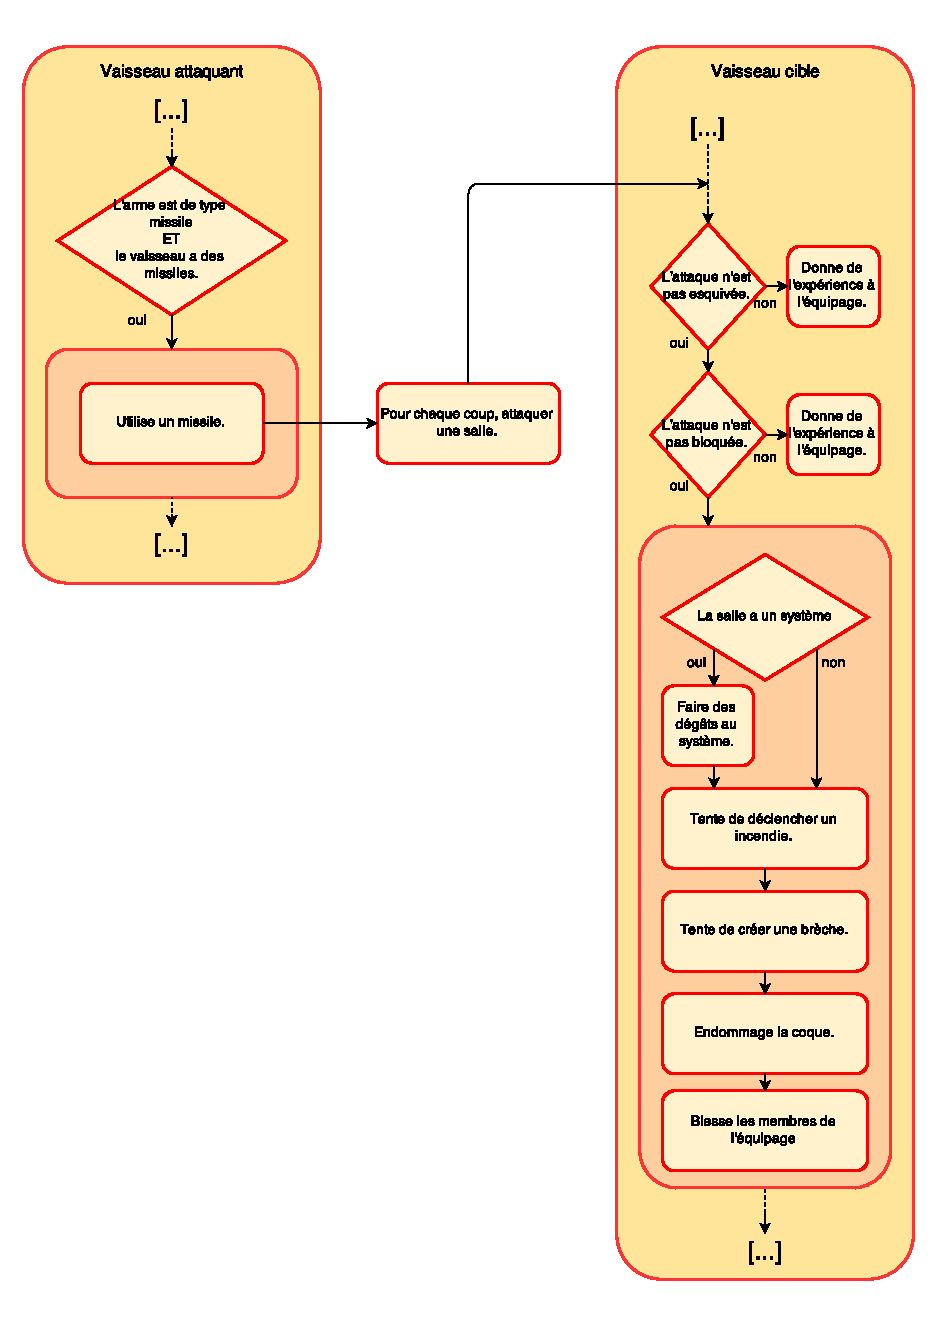
\includegraphics[width=1.1\linewidth]{attackSequenceMissileLaser.pdf}
			\end{figure}
			Les armes lasers et missiles ont des fonctionnements similaires (figure~\ref{fig:missileAttackWeapon}). Seul le déclenchement de l'utilisation d'un laser est différent puisqu'il ne faut pas vérifier qu'il y a des missiles en stock et qu'il ne faut pas utiliser de missile lorsque l'attaque est déclenchée. Ensuite la même méthode du vaisseau adverse est appelée. \\
			Celle-ci manipule d'abord l'esquive et les boucliers. Ensuite, si l'attaque est passée, des dégâts sont appliqués aux systèmes, aux membres d'équipage présents dans la salle, à la coque et des départs de feu ou des brèches peuvent être générés. 
			\begin{figure}[H]
				\caption{Utilisation d'une arme à ion}
				\label{fig:ionAttackWeapon}
				\centering
				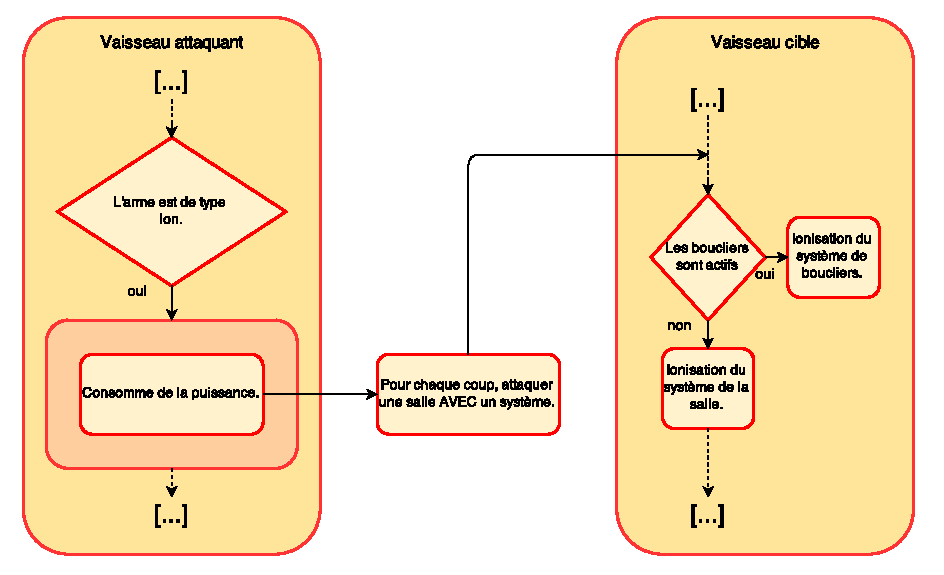
\includegraphics[width=1\linewidth]{attackSequenceIon.pdf}
			\end{figure}
			Les armes ions font des dégâts temporaires aux systèmes et seulement à eux (figure~\ref{fig:ionAttackWeapon}).\\
			Pour utiliser ces armes, il suffit donc d'appeler la méthode du vaisseau adverse. Celle-ci va juste se contenter de d'ioniser les boucliers s'il y a une couche de bouclier opérationnelle, sinon ioniser le système visé originellement.
			\begin{figure}[H]
				\caption{Utilisation d'une arme à rayon}
				\label{fig:beamAttackWeapon}
				\centering
				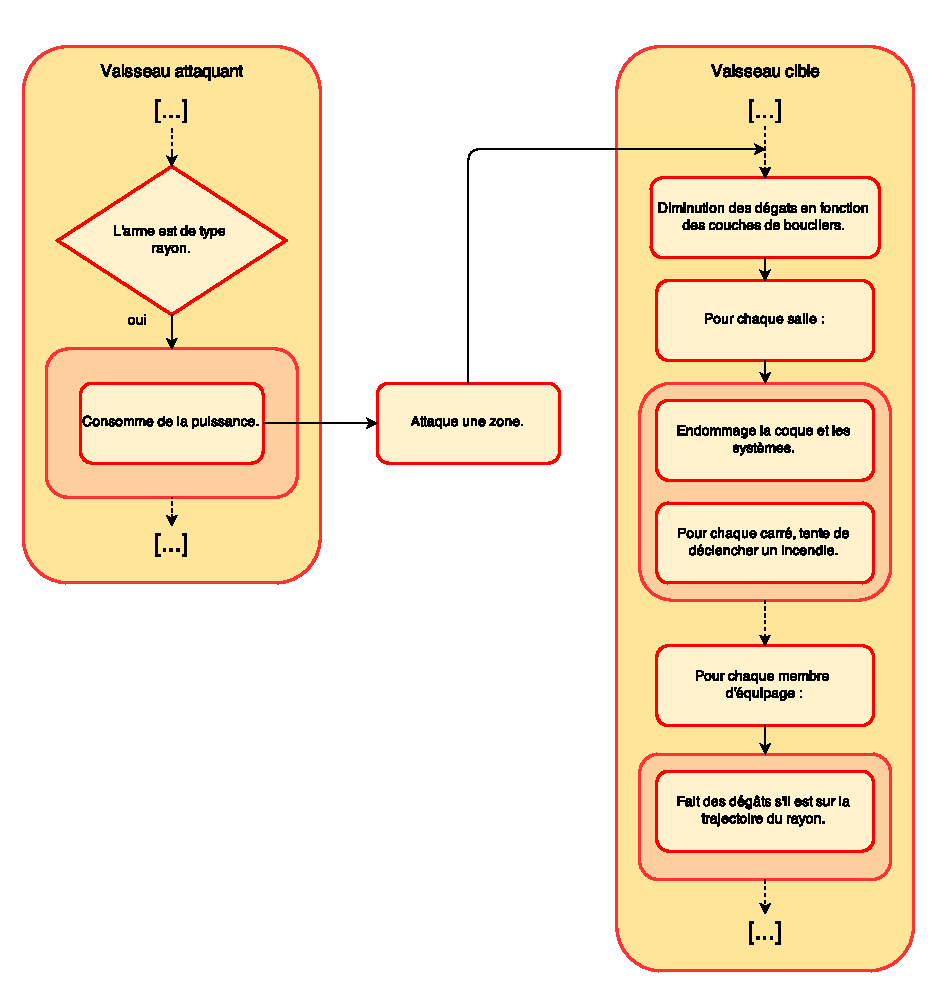
\includegraphics[width=1\linewidth]{attackSequenceBeam.pdf}
			\end{figure}
			Les rayons font des dégâts sur une ligne dans le vaisseau grâce à des coordonnées aléatoires (figure~\ref{fig:ionAttackWeapon}).\\
			La méthode du vaisseau adverse devra donc faire des dégâts à tout ce qui se trouve sur le chemin du rayon.

			\medskip

			\paragraph{L'utilisation d'un drone} 

			Les seuls drones gérés pour l'instant sont des drones d'attaque qui ont un comportement similaire à l'utilisation des armes. À chaque fois qu'ils sont rechargés et qu'ils sont activés par le système des drones, ils attaquent une cible déterminée de la même façon que pour les armes.

		\subsection{La gestion des cooldowns}

			\paragraph{Le vaisseau}
			L'ordre des différentes instructions n'a pas vraiment d'importance. Nous allons donc lister ces instructions : \\
			\begin{enumerate}
				\item Demander aux systèmes de gérer leurs cooldowns.
				\item Essayer d'alimenter les différents systèmes, armes et drones.
				\item Annuler les réparations effectuées d'un système s'il n'y a plus personne dans la salle. (Ce fonctionnement n'est pas optimal et pourrait être changé si les membres d'équipage se déplaçaient car dès qu'un membre quitte une salle on pourrait déclencher la remise à zéro des réparations)
				\item Demander aux salles de gérer leurs cooldowns.
				\item Demander aux membres d'équipage de gérer leurs déplacements (cette partie ne fonctionnant pas très bien, et n'étant pas la priorité du programme, nous avons décidé de mettre cet élément du jeu en pause).
				\item Ajouter de l'oxygène aux salles grâce au système.
				\item Essayer d'utiliser l'invisibilité.
			\end{enumerate}

			\medskip

			\paragraph{Les systèmes}
			Tous les systèmes doivent gérer le cooldown de leur ionisation.\\
			Le système des boucliers doit gérer le cooldown de ses couches de bouclier.\\
			Les systèmes des armes et des drones doivent recharger respectivement les armes et les drones.
			\medskip

			\paragraph{Les salles}
			\begin{enumerate}
				\item Gérer les différentes tâches des membres d'équipage présents (réparation, extinction...).
				\item Gérer les dégâts faits aux membres d'équipage.
				\item Gérer le reste de l'oxygène.
				\item Gérer les feux et les brèches.
			\end{enumerate} 

	\section{La discrétisation des évènements}

	Cette gestion des attaques et des cooldowns implique qu'à chaque tour le vaisseau vérifie plusieurs tests, incrémente des compteurs, etc. Cela prend du temps et n'est forcément utile. 
Pour éviter cela, nous avons discrétisé certains évènements. Cela consiste à avoir une file d'évènements (implémentée sous la forme d'une liste) dont les évènements de la tête sont effectués durant un tour et on supprime ensuite la tête pour avoir les évènements suivants au tour suivant.

	Dans le moteur de combats, chaque vaisseau a deux listes d'évènements, une pour les attaques et une pour les cooldowns. Parmi les évènements discrétisés il y a :
	\begin{itemize}
		\item l'utilisation des drones ;
		\item l'utilisation de l'invisibilité ;
		\item l'ionisation des systèmes.
	\end{itemize}

	Au final, peu d'évènements ont été discrétisés car la plupart des évènements gérés par notre moteur de combats ont des interactions régulières avec d'autres éléments du vaisseau. Par exemple, le rechargement des armes est affecté par la présence ou non d'un membre d'équipage, donc à chaque tour il faudrait vérifier si un membre d'équipage est présent et vérifier son niveau, pour ensuite déplacer le rechargement de l'arme dans la liste d'évènements ce qui prend du temps. Ces cas sont communs chez les évènements de base du jeu originel, or notre moteur de combats est composé en grande partie par les aspects basiques du jeu, cela explique donc la petite utilisation de la discrétisation des évènements. De plus, si le moteur de combats est enrichi avec des évènements avancés et donc avec peu d'interactions, le temps moyen d'un combat n'augmentera presque pas.

	\section{Représentation graphique}
	
	Optionnellement, nous avons ajouté un système de représentation graphique d'un combat entre deux vaisseaux. En effet cet ajout ne sert pas à l'exploitation des données, et nous permet simplement d'obtenir un aperçu graphique d'un duel. Ces aperçus sont faits grâce à la librairie python \textit{tkinter}.
	
	\begin{figure}[H]
		\caption{Une image regroupée des deux vaisseaux à un temps donné}
		\label{fig:imgMagick}
		\centering
		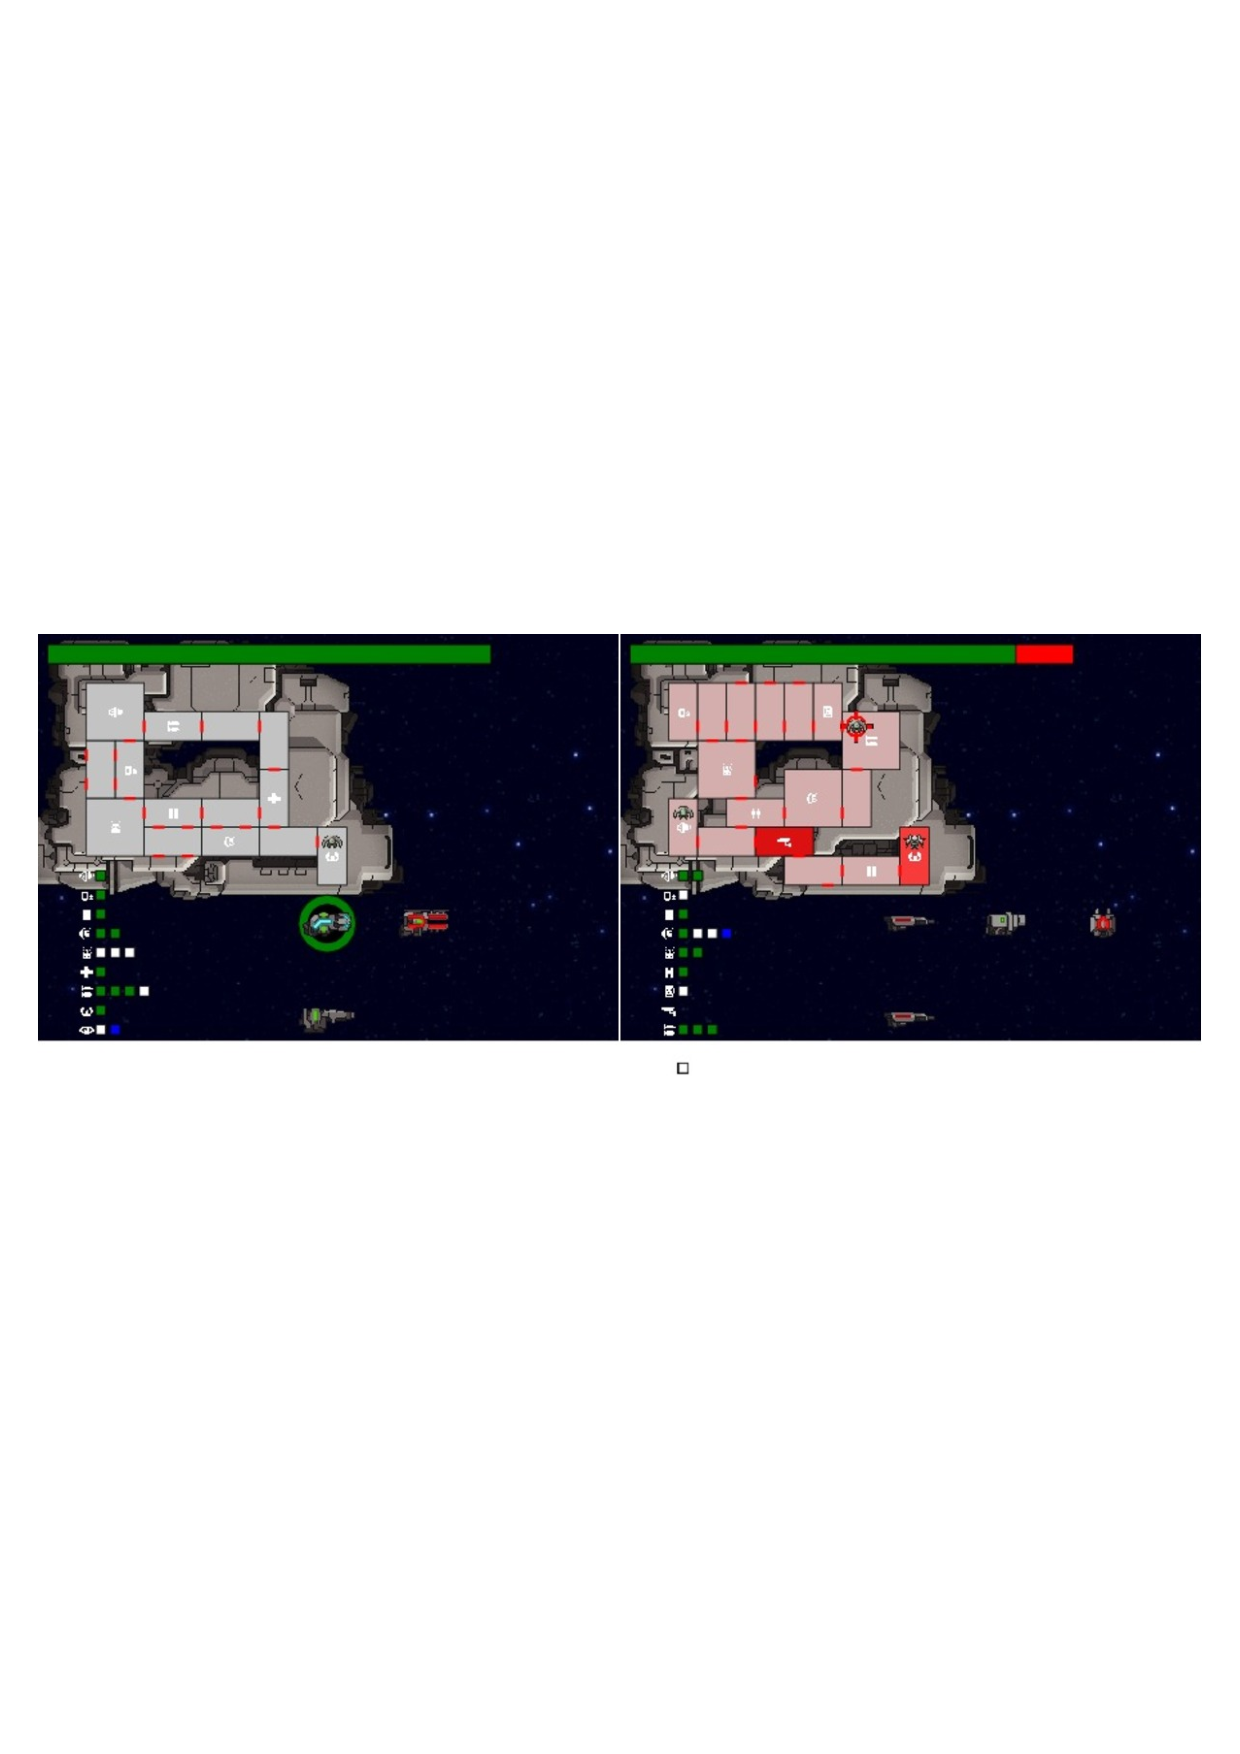
\includegraphics[angle=90,scale=0.765]{imageMagick.pdf}
	\end{figure}
	
	Malheureusement l'utilisation que nous voulions en faire en départ n'a pas pu être fait comme nous le souhaitions. En effet, de base nous voulions que le combat s'affiche dans une fenêtre qui s'updaterait. Cependant la personnalisation des classes des fenêtres tkinter ne permet pas l'affichage qui nous permet de faire cela (ou en tout cas, nous n'avons pas réussi à comprendre pourquoi ces affichages ne fonctionnaient pas).
	C'est pourquoi nous avons opté pour une seconde méthode, un peu plus longue. C'est le fichier scriptps.sh qui permet cela.
	
	\begin{enumerate}
		\item Dans un premier temps, un combat est lancé.
		\item Pour chaque action, et chaque vaisseau, une fenêtre tkinter s'ouvre présentant l'état des deux vaisseaux.
		\item Un fichier postscript est extrait de chaque fenêtre tkinter.
		\item Chaque fichier postscript est transformé en jpg
		\item Toutes les images jpg sont regroupées par deux, regroupant ainsi les deux vaisseaux à un temps donné. (figure~\ref{fig:imgMagick})
		\item Enfin, toutes les images sont regroupées en un seul gif.
	\end{enumerate}
	
	Toutes les manipulations d'images sont faites par le script bash utilisant le logiciel ImageMagick
	
	\section{Diverses techniques de jeu}
	
	\paragraph{Buffer} Cette technique consiste à avoir le niveau d'un système plus haut que nécessaire pour qu'une ionisation ou que des dégâts faits au système ne soient pas trop handicapants car le fonctionnement du système touché ne sera pas affecté.
